% %!TEX root = ../main.tex
\chapter{Methodology}
\label{chp:methodology}

In this chapter, we provide a formal definition of the problem of joint entity and relation extraction in section \hyperref[sec:probdef]{[3.1]}. Then, in section \hyperref[sec:approach]{[3.2]}, we describe our approach in detail. First explaining the entity model in section \hyperref[sec:entitymodel]{[3.2.1]}, and then describing the relation model in section \hyperref[sec:relationmodel]{[3.2.2]}. Finally, we explain the training and inference processes in section \hyperref[sec:relationmodel]{[3.2.3]}.
\section{Problem Definition}
\label{sec:probdef}
Given \(X\) an input sentence consisting of \(n\) tokens \(x_1,x_2,...,x_n\). Let \(S = {s_1, s_2,...,s_m}\) be all the possible spans in \(X\) of up to length \(L\) and \(START(i)\) and \(END(i)\) denote start and end indices of \(s_i\). The problem can be decomposed into two sub-tasks:

\textbf{Named entity recognition} Let \(E\) denote a set of pre-defined entity types. The named entity recognition task is, for each span \(s_i \in S\), to predict an entity type \[y_e(s_i) \in E\] or, span \(s_i\) is not an entity: \[y_e(s_i) =\epsilon\]

The output of the task is \[Y_e = {(s_i , e) : s_i \in S, e \in E}\].


\textbf{Relation extraction} Let \(R\) denote a set of predefined relation types. The task is, for every pair of spans \(si \in S\), \(sj \in S\), to predict a relation type \[y_r(s_i , s_j ) \in R\], or there is no relation between them: \[y_r(s_i , s_j ) =\epsilon\]. The output of the task is \[Y_r = {(s_i , s_j , r) : s_i , s_j \in S, r \in R}\].

\section{Our Approach}
\label{sec:approach}

We based our approach on the state of the art proposed by Zhong et al. \cite{Zhong2020AFE}. The simplicity of their model and its performance make it a prime candidate for NER and RE on new datasets. Therefore we first reproduced their results on the SciERC dataset. Then, we prove that their model can be generalized to other datasets. In the next chapter, we will dive deeper into our experiments and demonstrate how we trained and evaluated their model on new NER and RE datasets. Namely the NYT \hyperref[sec:nytdataset]{[2.2.3.1]} and TACRED\hyperref[sec:tacreddataset]{[2.2.3.2]} datasets. The goal is to have a framework that, given any NER and RE dataset, can be easily used to train NER and RE models.\\

\subsection{Entity model}
\label{sec:entitymodel}
The entity model is inspired by previous research (Lee et al. \cite{lee-etal-2017-end}; Luan et al. \cite{luan-etal-2019-general}; Wadden et al. \cite{Wadden2019EntityRA}). It begins by using a pre-trained language model, such as BERT, to understand the context of each word in a sentence. For any given segment of text, known as a 'span', we create a context representation \(\text{x}_t\) for each input token \(x_t\). This is done by combining the context of the span's first and last words with additional features that capture the span's length. We then use this combined information to calculate the likelihood of each possible entity type that this span could represent.\\
Formally, Let \(S\) be an input sentence, and \(s_i\) a span of \(S\)  \(s_i \in S\), we can define the span representation \(h_e(s_i)\) as\cite{Zhong2020AFE}: \[h_e(s_i) = [x_{START(i)} ; x_{END(i)} ; \phi(s_i)]\], where \(\phi(s_i) \in R^d_F\) is a representation of the span width features. Finally, \(h_e(s_i)\) becomes the input to a \ac{FFN} that will predict the entity type. Or, more precisely, its probability distribution: \[e \in E \cup {\epsilon}: P_e(e | s_i)\].

\subsection{Relation Model}
\label{sec:relationmodel}
The relation model function is to take two spans \(s_i\) , \(s_j\), which are the 'subject' and 'object' as input and output a relation between them. Or output \(\epsilon\) if there's no relation. Most works we examined (Luan et al. \cite{luan-etal-2019-general}; Wadden et al. \cite{Wadden2019EntityRA}) use the same span representations \(h_e(s_i)\), \(h_e(s_j)\) in the relation model to predict the relation between \(s_i\) and \(s_j\) . Hover, Zhong et al. \cite{Zhong2020AFE} suggest that while these representations can understand the context surrounding each entity independently, they might not effectively identify the connections or relationships between pairs of text segments. They also point out that using the same contextual information for different pairs of text segments might not always be the best approach. For example, the phrase "is a" is important for recognizing the relationship between MORPA and PARSER in Figure 1, but does not help in understanding the connection between MORPA and TEXT-TO-SPEECH.

\begin{figure}[ht]
    \centering
    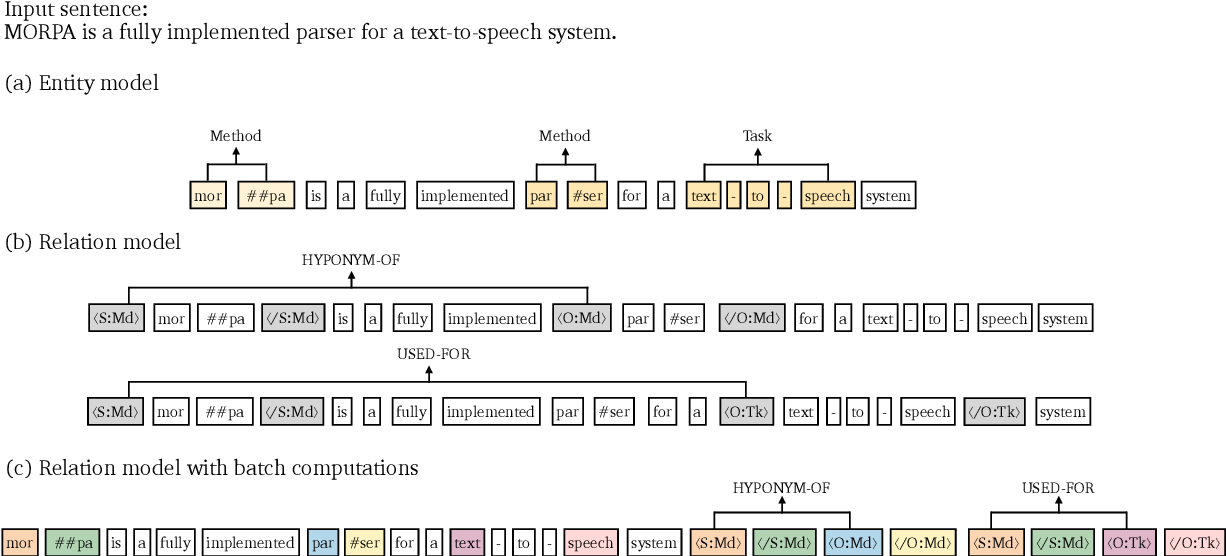
\includegraphics[width=1\textwidth]{figures/figure1.png}
    \caption{An input sentence from the SciERC dataset. Luan et al. \cite{luan-etal-2019-general}}
    \label{fig:examplefromsciercdataset}
\end{figure}

Instead, Zhong et al. \cite{Zhong2020AFE} propose a relation model that looks at each pair of spans separately and adds specific markers in the initial processing stage. These markers indicate which span is the subject and which is the object, as well as their types, to improve the model's understanding. Formally, Let \(X\) be an input sentence and \(s_i\) , \(s_j\) be a pair of subject-object spans and \(ei , ej \in E \cup {\epsilon}\) are their types respectively. Then we define text markers as \(\langle S:e_i\rangle\), \(\langle /S:e_i\rangle\), \(\langle O:e_j\rangle\), and \(\langle /O:e_j\rangle\), and embedded them into \(X\) before and after \(s_i\) and \(s_j\) (Figure 1 (b)). Let \(\widehat{X}\) be the new sequence after inserting the markers: \[\widehat{X} = ...\langle S:e_i\rangle,x_{START(i)},...,x_{END(i)},\langle /S:e_i\rangle\,...\langle /O:e_j\rangle,x_{START(j)},...,x_{END(j)}\langle /O:e_j\rangle\]

Next, we use another pre-trained encoder on \(\widehat{X}\) and we refer to its output representations with by \(\widehat{x}_t\). We combine the outputs from their starting points to understand the relationship between the two spans. This gives us a combined representation: \[h_r(s_i,s_j)=[{\widehat{x}}_{\widehat{START(i)}};{\widehat{x}}_{\widehat{START(j)}}]\]
where \(\widehat{START(i)}\) and \(\widehat{START(j)}\) are the indices of \(\langle S:e_i\rangle\) and \(\langle O:e_j\rangle\) in \(\widehat{X}\). Finally, \(h_r(s_i,s_j)\) will be the input to an FFN that will predict the relation between \(s_i\) and \(s_j\): \[r \in R \cup {\epsilon}: P_r(r|s_i , s_j )\].

The approach of using special markers to identify subjects and objects in a text is not particularly novel and has been explored before in classification studies (Zhang et al.\cite{zhang-etal-2019-ernie}; Soares et al.\cite{baldini-soares-etal-2019-matching}; Peters et al.\cite{peters2019knowledge}). However, these studies usually focus on classifying the relationship between one pair of subjects and objects within a sentence Zhang et al.\cite{zhang-etal-2017-position}, such as in the TACRED dataset\hyperref[sec:tacreddataset]{[2.2.3.2]}. The effectiveness of this method has not been fully tested in the end-to-end setting like the Zhong et al. \cite{Zhong2020AFE} hope to classify the relations amongst more entity mentions. They saw a significant improvement in their solution, strengthening the idea that different context-aware representations are invaluable for understanding the relations between entities pairs in one example.. Furthermore, Zhang et al.\cite{zhang-etal-2019-ernie}; Soares et al.\cite{baldini-soares-etal-2019-matching} used untyped only markers (e.g., \(\langle S:\rangle\), \(\langle /S:\rangle\)) and previous end-to-end models (e.g., (Wadden et al.\cite{Wadden2019EntityRA})) only inject the entity type information into the relation model through auxiliary losses. Zhong et al. \cite{Zhong2020AFE} found that injecting type information at the input layer is very helpful in distinguishing entity types — for example, whether “Disney” refers to a person or an organization— before trying to understand the relations.

\subsection{Training and Inference}
\label{sec:trainingandinference}
We adapt two pre-trained language models by fine-tuning them with task-specific loss functions, employing cross-entropy loss\cite{Zhong2020AFE}, for both the entity and relation extraction models. This equation penalizes the model more heavily when its predicted probability for the true entity type is lower, encouraging the model to correctly recognize entity types.
\[\mathcal{L}_e=-\sum_{s_i\in S}\log{P_e(e_i^*|s_i)}\]
Where \(\mathcal{L}_e\) represents the cross-entropy loss function for the entity model. It is calculated by summing the negative log probabilities of the true (gold) entity types (\(e_i^*\)) for all spans (\(s_i\)) in the dataset (\(S\)). The probability \(P_e(e_i^*|s_i)\) reflects how likely it is that the span \(s_i\) corresponds to its gold entity type \(e_i^*\) according to the model.
\[\mathcal{L}_r=-\sum_{s_i,s_j\in S, s_i \neq s_j}\log{P_r(r_{i,j}^*|s_i,s_j)}\]
Where \(\mathcal{L}_r\) represents the cross-entropy loss function for the relation model. Similar to \(\mathcal{L}_e\), this loss function sums the negative log probabilities that the model assigns to the true (gold) relation types (\(r_{i,j}^*\)) between pairs of spans (\(s_i,s_j\)) in the dataset (\(S\)), where \(s_i \neq s_j\). The probability \(P_r(r_{i,j}^*|s_i,s_j)\) indicates the model's confidence that the correct relation between the spans \(s_i\)and  \(s_j\) is \(r_{i,j}^*\).

where \(e_i^*\) represents the gold entity type of \(s_i\) and \(r_{i,j}^*\) represents the gold relation type of span pair \(s_i,s_j\) in the training data. For training the relation model, we only consider the gold entities \(S_G \subset S \) in the training set and use the gold entity labels as the input of the relation model. During inference, we first predict the entities by taking \(y_e(s_i) = arg max_{e \in \varepsilon \cup \{\epsilon\}} P_e(e|s_i)\). Denote 
\(S_{pred} = {s_i:y_e(s_i) \neq \epsilon}\), 
we enumerate all the spans \(s_i , s_j \in S_{pred}\) 
and use \(y_e(s_i), y_e(s_j)\) to construct the input for the relation model \(P_r(r|s_i,s_j )\).

In training the relation model, we focus exclusively on the spans marked as entities according to the gold standard \(S_G\), which is a subset of all spans \(S\) in the dataset (\(S_G \subset S\)). This allows the model to learn from the most relevant examples, using the gold entity labels to understand relationships within the text.

During the inference phase, the model predicts entities by determining the most likely entity type for each span \(s_i\). That's done by taking \[y_e(s_i) = arg max_{e \in \varepsilon \cup \{\epsilon\}} P_e(e|s_i)\], where \(\varepsilon\) includes all possible entity types and \(\epsilon\) indicates a non-entity. Spans not identified as entities are filtered out, creating a set \(S_{pred} = {s_i:y_e(s_i) \neq \epsilon}\) of spans predicted to be entities.

With \(S_{pred}\) established, the model then examines every possible pair of spans within it to predict their interrelations. For each span pair \(s_i,s_j \), it employs the predicted entity types as inputs to the relation model \(P_r(r|s_i,s_j )\). This step utilizes the insights gained from entity prediction to enhance the accuracy of relation extraction, aiming to comprehensively map out the network of relationships among identified entities in the text. This process underscores the model's integrated approach, leveraging entity predictions to inform and refine relation extraction, thus creating a cohesive understanding of the textual content.